\section{Parallel Huffman Implementation}
To parallelize our algorithm over threads and processes, we decided to follow this simple yet effective structure
\begin{itemize}
    \item multiple processes will process groups of file and folders separately.
    \item multiple threads of the same process will compute different chunk of the same file in parallel.
\end{itemize}

There are a many reasons to our choice. Mainly they are:

\begin{itemize}
	\item In most operating systems a file is a resource that the OS gives to a single process. We wanted to follow a similar design philosophy.
	\item Most operating system can allow multiple processes to open the same file in reading mode, but few allow to multiple processes to open the same file in writing mode. This is because that leads to potentially concurrency and data integrity issues. By having only a single process open a single file, we avoid all these issues.
	\item Because threads of the same process share the address space, we can avoid the expensive data transfer across processes. When data is read or written to file, there is no need to transfer data between threads.
\end{itemize}

We start by explaining the basic multithreading operations on a single file and then we'll cover multiprocessing with multiple files.

\subsection{Multithreading}

The parallel algorithm for a single file follows the same exact procedure as a serial version, but with few key differences to allow multithreading.

A single file is divided in chunks of a fixed size. When that is done, the single process forks and creates the number of threads we intented.

One of them reads a number of chunks equal to the team size. When it's done reading the chunks, all threads can work on the processing in parallel. 

Every chunk is processed by a single thread, that reads and writes on the shared memory space of its process. Although all the chunks are in shared memory, each thread is assigned a single chunk and it processes only data in own chunk to avoid any concurrency related problems.

When all threads are done  computing either the encoding or decoding of their chunks, a single thread writes the processed chunks to the output file.
Again, because all threads share a memory space there is no need to perform data transfer.


The overall procedure is the same in both encoding and decoding, with very small differences. 

We also parallelized the counting of occurences of a byte in the input file, that is required in order to create the huffman tree, with a similar architecture.  Key difference is that there is no output file to write, but only occurences to count.

In figure \ref{fig:threading}a schema of the architecture. 

\begin{figure}
	\centering
	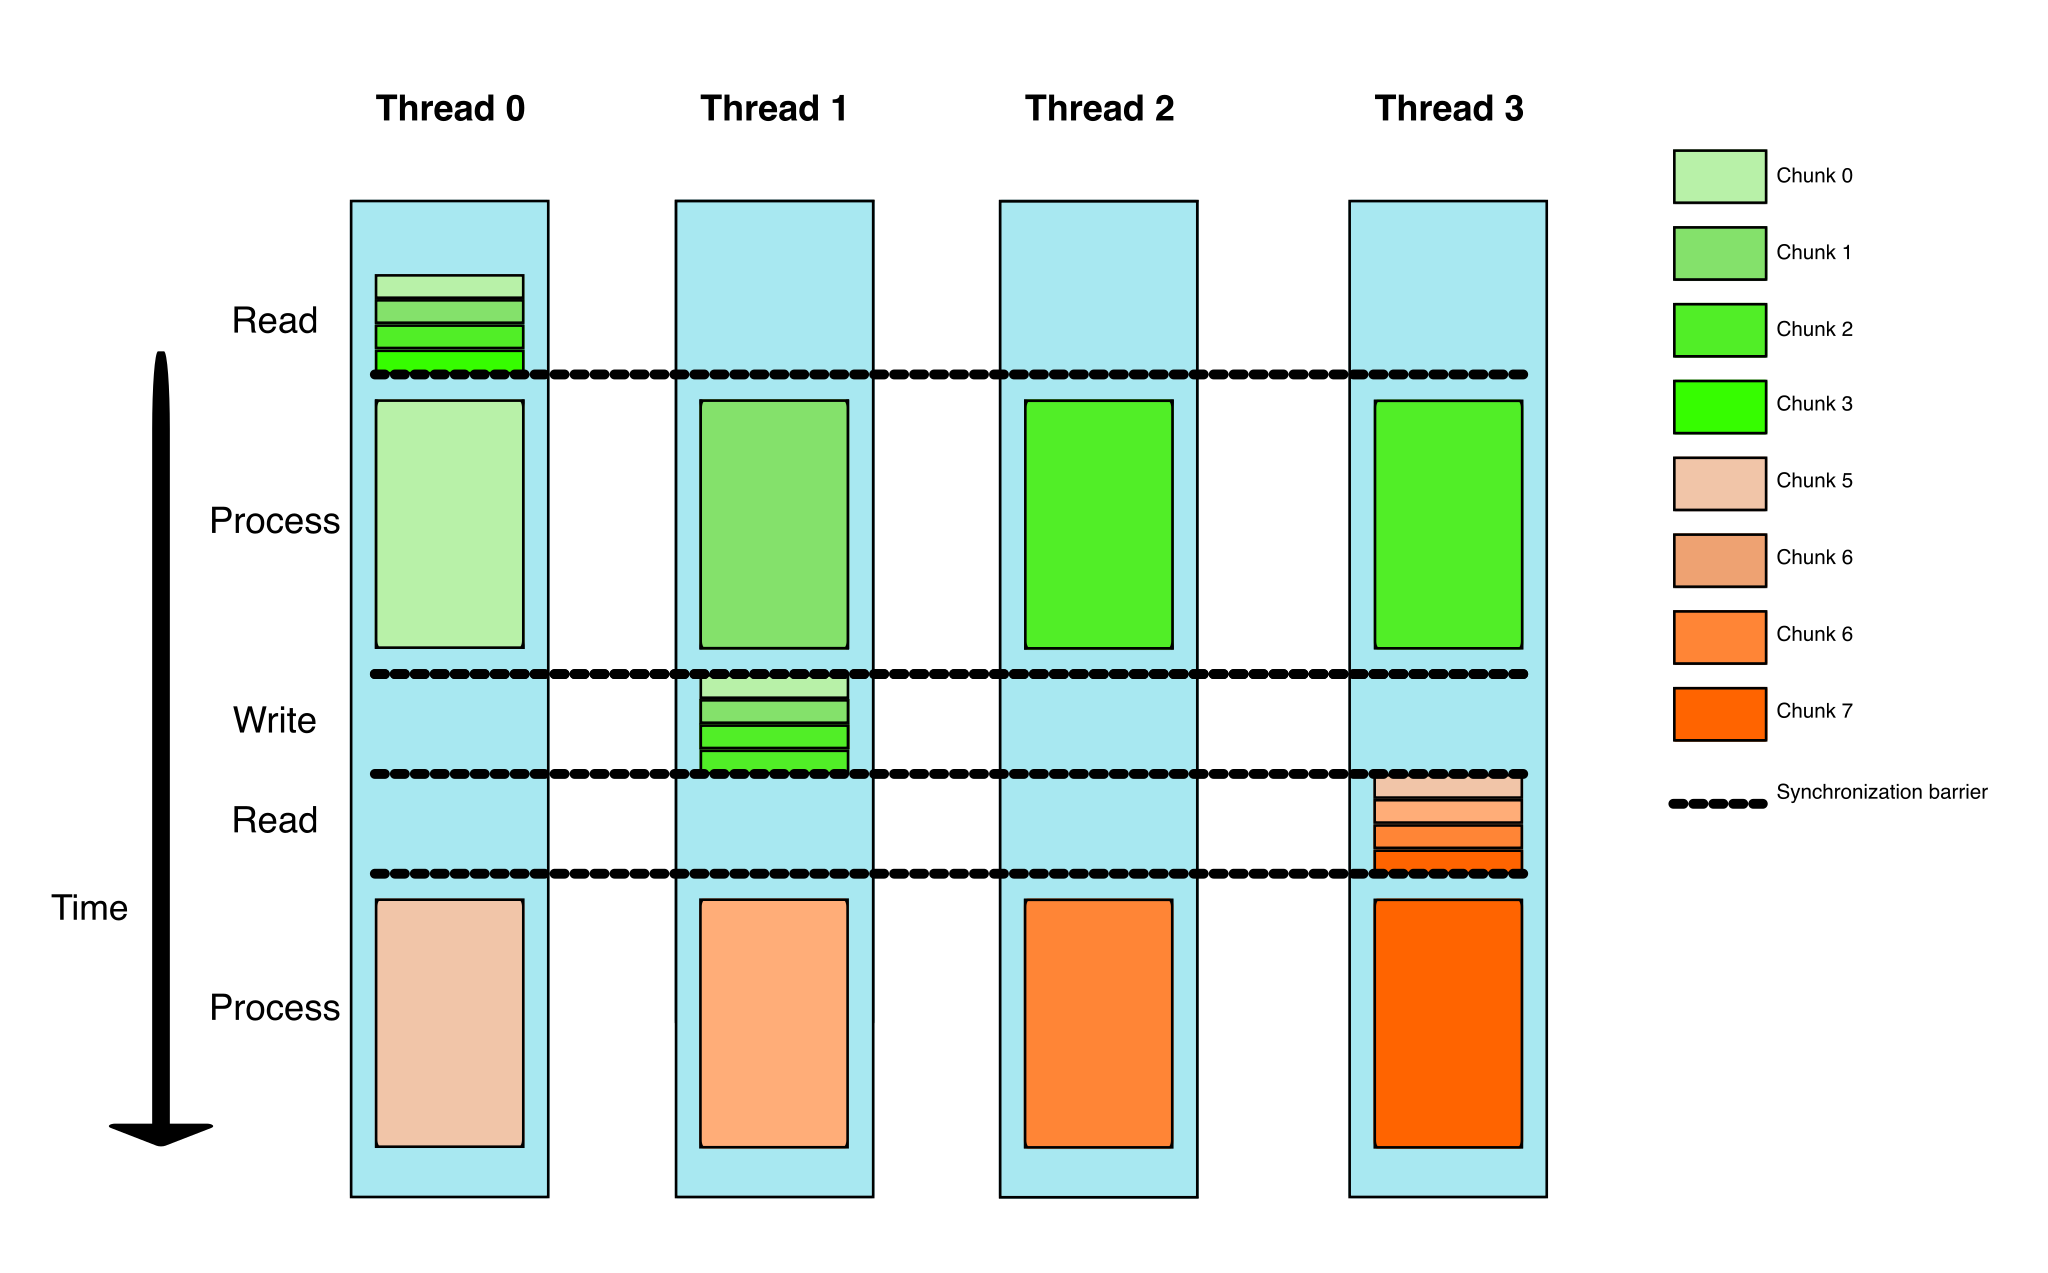
\includegraphics[width=0.8\linewidth]{../imgs/threading}
	\caption{Simple schema of the threading paradigm.}
	\label{fig:threading}
\end{figure}


\subsection{Multiprocessing}

For multiple files we wanted to exploit multiprocessing.

To do this we devised a simple algorithm to distribuite files across multiple processes, so that each process can work on its own list of files, indipendently to others. This way we can minimize communcation and therefore latency and other slowdowns.


First of all the process with rank 0 crawls all the files present in the input directory recursively. Then it opens all the files and reads their size.

Once all files and their respective sizes are known, process 0 creates  a min priority queue where each item represents a process and its priority is the  size of files that have been assigned to it.

Process 0 can iteratively insert files in the priority queue and updates the priority of each process with the cumulative file size. The main idea is that we can ensure an equal work division among different processes. 

When all this is done, process 0 sends the list of files to each process and then each starts to work indipendetly on its own list of files.



\subsection{Implementation details and other notes}

\begin{itemize}

\item We found that a chunk size of 4096 Byte had the best I/O times. This is probably due to the fact that 4096 B is the size of a page in most Linux based operating systems. The last chunk of a file may be smaller. Reading any other size at the time had resulted in significanlty worse I/O times ( both increasing and decreasing the chunk size ).

\item In general, all threads will finish processing their chunk at around the same time, but in some cases, there are threads that can take longer. This is due to the very unlucky case where a whole chunk contains exclusively very infrequent characters or bytes of data. Because the bytes are very infrequent each is encoded in extremely long sequences, up to 256 bits, resulting in a bigger encoded chunk than compared to the original data. With our alphabet at 1 Byte, the worst case results in a chunk that is 32 times bigger than original.

\item We tried to parallelize the I/O, by having each thread read its own chunk. We found that the standard file descriptor provided by C have a lock to guarantee thread safety.  This lock slows down the reads significantly. We also tried using multiple file descriptors to circumvent this limitation, however we found no improvement over a sequential read done by one thread for all the threads in it's team. This is likely because the O.S. schedules I/O requests and serves them one at the time, resulting in a impossiblity of having truly parallel I/O.

\item We also tested an architecture where we had two dedicated threads to I/O, one for reading and one for writing chunks. The idea is that whenever a chunk is processed, the I/O threads would immediately write the processed chunk to the output file and similarly a new chunk would be read from the input file. Theoretically this would allow to parallelize I/O and computation operations and we avoided concurrency problems by synchronizing the I/O with locks. However we found that this approach was a waste  of resources, as the I/O on the cluster is extremely fast ($\sim$ 5 GiB +/s) and it resulted in the I/O threads being idle most of the time, waiting for a chunk to be processed. Although we discarded this architecture, it may be useful in systems or problems where I/O operations take a significant amount of time or at least comparable to processing operations. 
\item Another noticeable detail we noticed on the implementation with two dedicated threads for I/O, is that if there are not enough cores on the CPU or if the operating system decides to allocate all the threads on a single processor, the encoding and decoding times are greatly affected by the scheduler. This is because it might be that the O.S. gives priority to threads that are waiting ( for example the writer cannot write any block until the first has finished, even if all others have finished)

\end{itemize}
